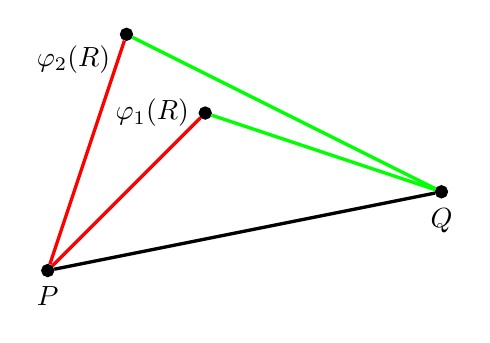
\begin{tikzpicture}
    \tikzstyle{point}=[circle,thick,draw=black,fill=black,inner sep=0pt,minimum width=4pt,minimum height=4pt]
    \node (P)[point,label={[label distance=0cm]-90:$P$}] at (0,0) {};
    \node (Q)[point,label={[label distance=0cm]-90:$Q$}] at (5,1) {};
    \node (A)[point,label={[label distance=0cm]180:$\varphi_1(R)$}] at (2,2) {};
    \node (B)[point,label={[label distance=0cm]190:$\varphi_2(R)$}] at (1,3) {};

    \draw[very thick] (P) edge node  {} (Q);
    \draw[very thick, red] (P) edge node {} (A);
    \draw[very thick, red] (P) edge node {} (B);
    \draw[very thick, green] (Q) edge node {} (A);
    \draw[very thick, green] (Q) edge node {} (B);
\end{tikzpicture}
